\documentclass[11pt,a4paper]{scrartcl}

\usepackage{fullpage}

%\usepackage[ngerman]{babel}
\usepackage[utf8]{inputenc}
\usepackage{graphicx}

\usepackage{amsmath}
\usepackage{amsthm}
\usepackage{mathtools}

\usepackage{listings}
\usepackage{xcolor}

%%%%% COMMANDS

\newcommand{\FT}{\mathcal{F}}
\newcommand{\T}{\mathrm{T}}
\newcommand{\IFT}{\mathcal{F}^{-1}}
\newcommand{\conv}{\ast}
\newcommand{\defined}{\coloneqq}

\newtheorem*{theorem}{Theorem}

\begin{document}

\lstdefinestyle{customc}{
    belowcaptionskip=1\baselineskip,
    breaklines=true,
    xleftmargin=\parindent,
    language=Python,
    showstringspaces=false,
    basicstyle=\footnotesize\ttfamily,
    keywordstyle=\bfseries\color{green!40!black},
    commentstyle=\itshape\color{purple!40!black},
    identifierstyle=\color{blue},
    stringstyle=\color{orange}
}
\lstset{
    style=customc
} 

\title{Image Analysis Excercise Sheet 7}
\author{Markus Doering, 3153320}
\maketitle

\section{Natural Image Statistics}
All python code for this excercise is found in file \verb$ia_07_01.py$ and in the appendix. 

In figure \ref{fig:1} we can see the histograms for the gradients of 4 natural images. The histograms arer more heavy-tailed compared to a Gaussian because of the areas of no intensity change and the sharp edges 
that are present in natural images. There is no significant difference of $\delta/\delta x$ and $\delta/\delta y$ visible. This could be due to the fact that no edge orientation is really dominant, like in the 
first image, or that most edges are diagonal and counted in both histograms, like in the last image.

Suppose we have an image where each pixel $x_i$ is drawn independently from a normal distribution of mean $\mu$ and variance $\sigma^2$ ($x_i \sim \mathcal{N}(\mu,\sigma^2),\ \forall 1\leq i\leq n$). We assume that the image 
has only one row, but the result clearly extends to normal images as well. The horizontal gradient image has entries $g_i = x_{i+1}-x_i$ (with $x_{n+1} = 0$), and since the $x_i$ are independent we 
can express the distribution of the gradient pixels as $g_i\sim\mathcal{N}(0,2\sigma^2)$. Therefore, the gradient of the random image is, again, a random image with zero mean and twice the variance.

\begin{figure}[hb]\label{fig:1}
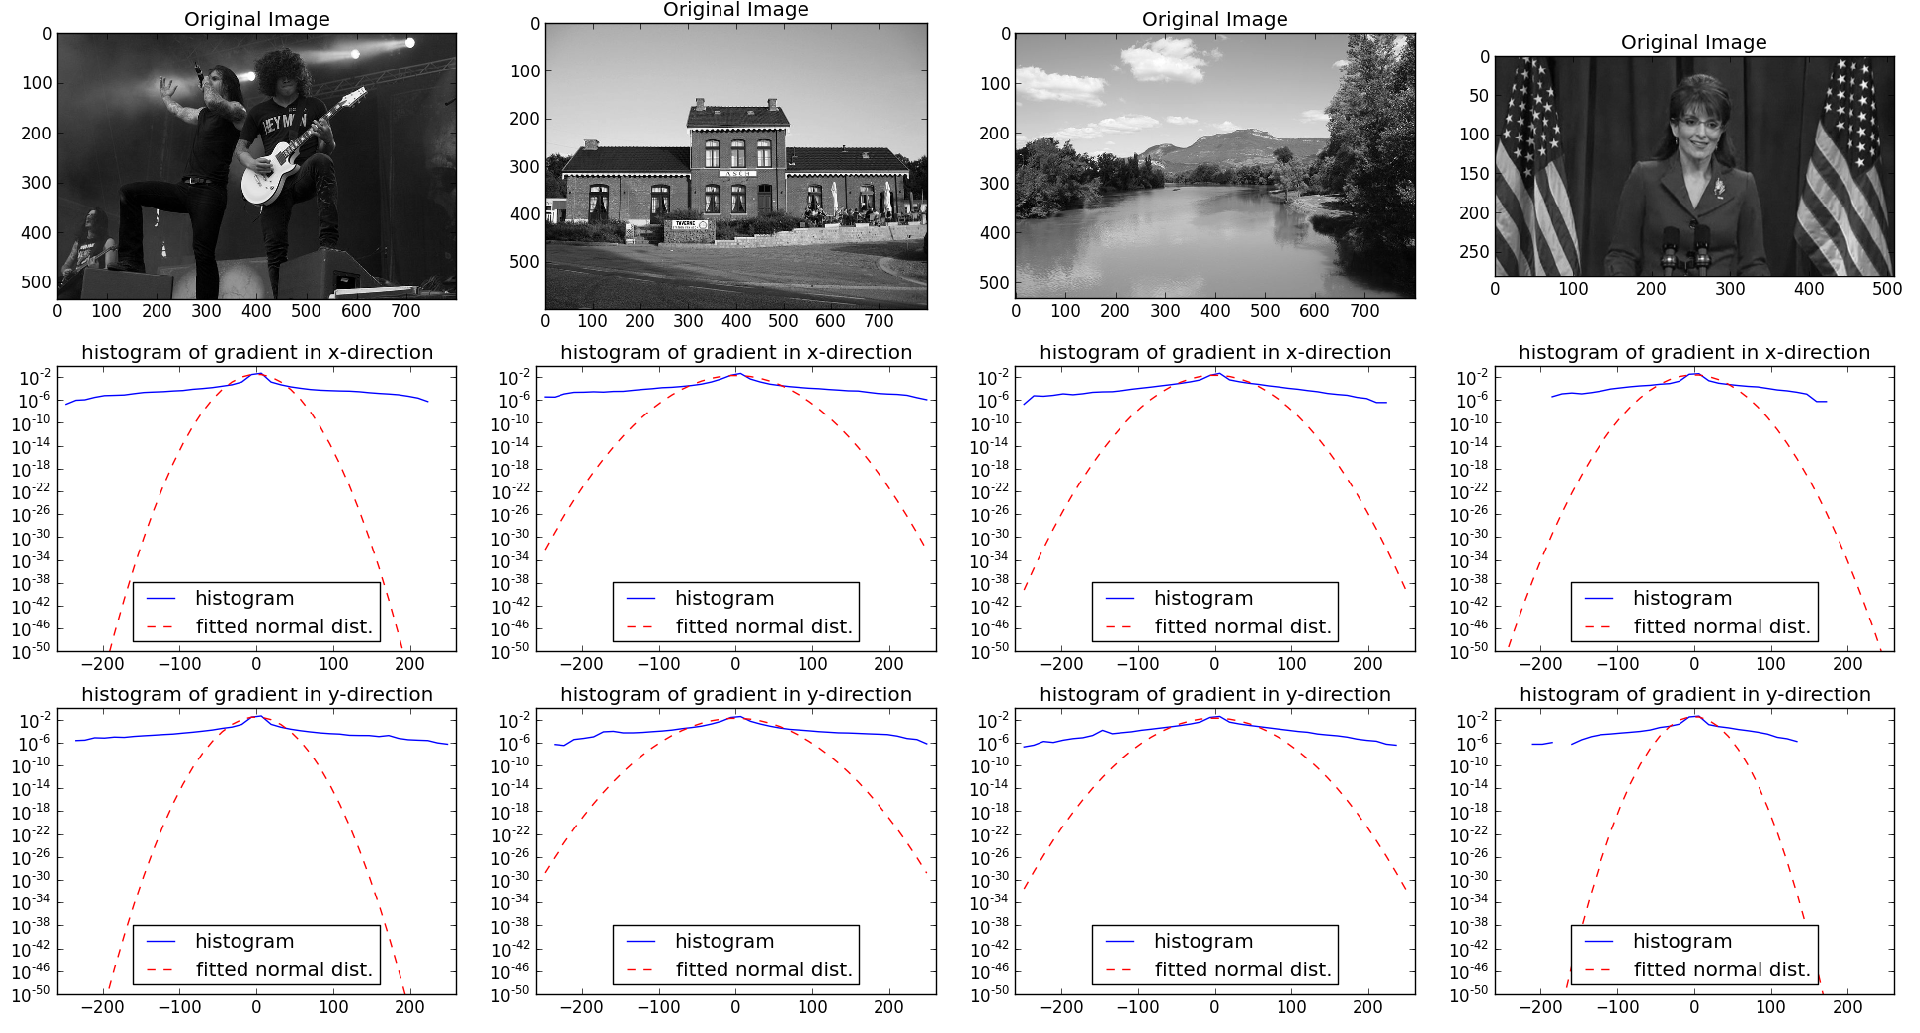
\includegraphics[width=.99\linewidth]{histograms_cut.png}
\caption{Natural images and the histograms of their gradients in x and y direction. The histograms are heavy-tailed compared to a Gaussian with equal mean and variance.}
\end{figure}

\stepcounter{section}
\section{Integer Linear Programming}
All python code for this excercise is found in file \verb$ia_07_03.py$ and in the appendix. 

In figure \ref{fig:3} we can see the solution to this excercise. The optimum of the ILP is the point $v_1=(3,2)$ with gain $g_1=18$, whereas the optimum of the LP is at the intersection of the red and the magenta line, 
$v_2\approx (2.4,3.4)$ with gain $g_2\approx19.8$. Rounding the LP solution to the closest integer point yields $v_3=(2,3)$ with gain $g_3=17$,  which is so far the worst solution.
\begin{figure}[hb]\label{fig:3}
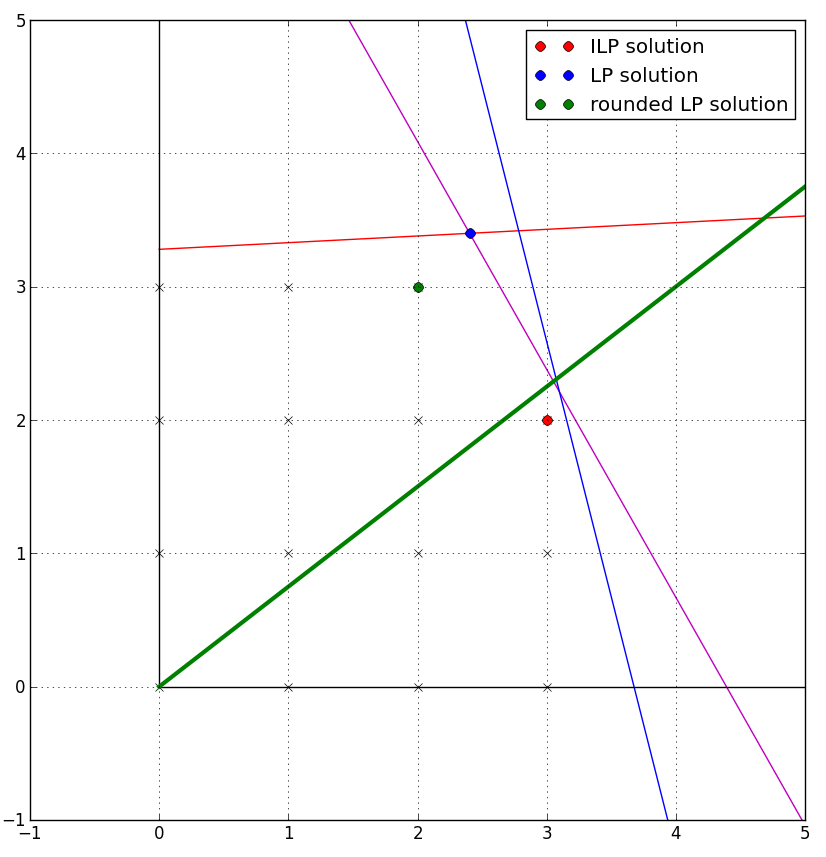
\includegraphics[width=.5\linewidth]{ex3_cut.png}
\caption{ILP diagram. The thin lines represent the constraints, the thick green line is the cost vector. }
\end{figure}

\clearpage
\appendix
\lstinputlisting[language=python]{ia_07_01.py}
\newpage
\lstinputlisting[language=python]{ia_07_03.py}
\end{document}